% Options for packages loaded elsewhere
\PassOptionsToPackage{unicode}{hyperref}
\PassOptionsToPackage{hyphens}{url}
%
\documentclass[
]{article}
\usepackage{amsmath,amssymb}
\usepackage{lmodern}
\usepackage{iftex}
\ifPDFTeX
  \usepackage[T1]{fontenc}
  \usepackage[utf8]{inputenc}
  \usepackage{textcomp} % provide euro and other symbols
\else % if luatex or xetex
       %%% MODIFIED: unicode-math conflics with expex; mathspects conflicts with glossaries/leipzig
  \usepackage{fontspec} % \usepackage{unicode-math}
  \defaultfontfeatures{Scale=MatchLowercase}
  \defaultfontfeatures[\rmfamily]{Ligatures=TeX,Scale=1}
  \setmainfont[]{DejaVu Sans}
\fi
% Use upquote if available, for straight quotes in verbatim environments
\IfFileExists{upquote.sty}{\usepackage{upquote}}{}
\IfFileExists{microtype.sty}{% use microtype if available
  \usepackage[]{microtype}
  \UseMicrotypeSet[protrusion]{basicmath} % disable protrusion for tt fonts
}{}
\makeatletter
\@ifundefined{KOMAClassName}{% if non-KOMA class
  \IfFileExists{parskip.sty}{%
    \usepackage{parskip}
  }{% else
    \setlength{\parindent}{0pt}
    \setlength{\parskip}{6pt plus 2pt minus 1pt}}
}{% if KOMA class
  \KOMAoptions{parskip=half}}
\makeatother
\usepackage{xcolor}
\IfFileExists{xurl.sty}{\usepackage{xurl}}{} % add URL line breaks if available
\IfFileExists{bookmark.sty}{\usepackage{bookmark}}{\usepackage{hyperref}}
\hypersetup{
  pdftitle={SQMB - Summative Assessment 1},
  pdfauthor={YOUR EXAM NUMBER},
  hidelinks,
  pdfcreator={LaTeX via pandoc}}
\urlstyle{same} % disable monospaced font for URLs
\usepackage[margin=1in]{geometry}
\usepackage{color}
\usepackage{fancyvrb}
\newcommand{\VerbBar}{|}
\newcommand{\VERB}{\Verb[commandchars=\\\{\}]}
\DefineVerbatimEnvironment{Highlighting}{Verbatim}{commandchars=\\\{\}}
% Add ',fontsize=\small' for more characters per line
\usepackage{framed}
\definecolor{shadecolor}{RGB}{248,248,248}
\newenvironment{Shaded}{\begin{snugshade}}{\end{snugshade}}
\newcommand{\AlertTok}[1]{\textcolor[rgb]{0.94,0.16,0.16}{#1}}
\newcommand{\AnnotationTok}[1]{\textcolor[rgb]{0.56,0.35,0.01}{\textbf{\textit{#1}}}}
\newcommand{\AttributeTok}[1]{\textcolor[rgb]{0.13,0.29,0.53}{#1}}
\newcommand{\BaseNTok}[1]{\textcolor[rgb]{0.00,0.00,0.81}{#1}}
\newcommand{\BuiltInTok}[1]{#1}
\newcommand{\CharTok}[1]{\textcolor[rgb]{0.31,0.60,0.02}{#1}}
\newcommand{\CommentTok}[1]{\textcolor[rgb]{0.56,0.35,0.01}{\textit{#1}}}
\newcommand{\CommentVarTok}[1]{\textcolor[rgb]{0.56,0.35,0.01}{\textbf{\textit{#1}}}}
\newcommand{\ConstantTok}[1]{\textcolor[rgb]{0.56,0.35,0.01}{#1}}
\newcommand{\ControlFlowTok}[1]{\textcolor[rgb]{0.13,0.29,0.53}{\textbf{#1}}}
\newcommand{\DataTypeTok}[1]{\textcolor[rgb]{0.13,0.29,0.53}{#1}}
\newcommand{\DecValTok}[1]{\textcolor[rgb]{0.00,0.00,0.81}{#1}}
\newcommand{\DocumentationTok}[1]{\textcolor[rgb]{0.56,0.35,0.01}{\textbf{\textit{#1}}}}
\newcommand{\ErrorTok}[1]{\textcolor[rgb]{0.64,0.00,0.00}{\textbf{#1}}}
\newcommand{\ExtensionTok}[1]{#1}
\newcommand{\FloatTok}[1]{\textcolor[rgb]{0.00,0.00,0.81}{#1}}
\newcommand{\FunctionTok}[1]{\textcolor[rgb]{0.13,0.29,0.53}{\textbf{#1}}}
\newcommand{\ImportTok}[1]{#1}
\newcommand{\InformationTok}[1]{\textcolor[rgb]{0.56,0.35,0.01}{\textbf{\textit{#1}}}}
\newcommand{\KeywordTok}[1]{\textcolor[rgb]{0.13,0.29,0.53}{\textbf{#1}}}
\newcommand{\NormalTok}[1]{#1}
\newcommand{\OperatorTok}[1]{\textcolor[rgb]{0.81,0.36,0.00}{\textbf{#1}}}
\newcommand{\OtherTok}[1]{\textcolor[rgb]{0.56,0.35,0.01}{#1}}
\newcommand{\PreprocessorTok}[1]{\textcolor[rgb]{0.56,0.35,0.01}{\textit{#1}}}
\newcommand{\RegionMarkerTok}[1]{#1}
\newcommand{\SpecialCharTok}[1]{\textcolor[rgb]{0.81,0.36,0.00}{\textbf{#1}}}
\newcommand{\SpecialStringTok}[1]{\textcolor[rgb]{0.31,0.60,0.02}{#1}}
\newcommand{\StringTok}[1]{\textcolor[rgb]{0.31,0.60,0.02}{#1}}
\newcommand{\VariableTok}[1]{\textcolor[rgb]{0.00,0.00,0.00}{#1}}
\newcommand{\VerbatimStringTok}[1]{\textcolor[rgb]{0.31,0.60,0.02}{#1}}
\newcommand{\WarningTok}[1]{\textcolor[rgb]{0.56,0.35,0.01}{\textbf{\textit{#1}}}}
\usepackage{longtable,booktabs,array}
\usepackage{calc} % for calculating minipage widths
% Correct order of tables after \paragraph or \subparagraph
\usepackage{etoolbox}
\makeatletter
\patchcmd\longtable{\par}{\if@noskipsec\mbox{}\fi\par}{}{}
\makeatother
% Allow footnotes in longtable head/foot
\IfFileExists{footnotehyper.sty}{\usepackage{footnotehyper}}{\usepackage{footnote}}
\makesavenoteenv{longtable}
\usepackage{graphicx}
\makeatletter
\def\maxwidth{\ifdim\Gin@nat@width>\linewidth\linewidth\else\Gin@nat@width\fi}
\def\maxheight{\ifdim\Gin@nat@height>\textheight\textheight\else\Gin@nat@height\fi}
\makeatother
% Scale images if necessary, so that they will not overflow the page
% margins by default, and it is still possible to overwrite the defaults
% using explicit options in \includegraphics[width, height, ...]{}
\setkeys{Gin}{width=\maxwidth,height=\maxheight,keepaspectratio}
% Set default figure placement to htbp
\makeatletter
\def\fps@figure{htbp}
\makeatother
\setlength{\emergencystretch}{3em} % prevent overfull lines
\providecommand{\tightlist}{%
  \setlength{\itemsep}{0pt}\setlength{\parskip}{0pt}}
\setcounter{secnumdepth}{5}
\ifLuaTeX
  \usepackage{selnolig}  % disable illegal ligatures
\fi

\title{SQMB - Summative Assessment 1}
\author{YOUR EXAM NUMBER}
\date{2023-02-22}

\begin{document}
\maketitle

\hypertarget{instructions}{%
\section{Instructions}\label{instructions}}

\textbf{PLEASE READ CAREFULLY}

\textbf{DUE THURSDAY 8 DECEMBER AT NOON}

Remember to include your \textbf{exam number as the author} in the
document preamble above.

Please, \textbf{use a sans-serif font}. I recommend the DejaVu Sans
font. You can download the DejaVu fonts here:
\url{http://sourceforge.net/projects/dejavu/files/dejavu/2.37/dejavu-fonts-ttf-2.37.zip}.

\textbf{Complete each exercise} by completing tasks, answering questions
and/or providing code if required.

\textbf{When you are ready to submit}:

\begin{enumerate}
\def\labelenumi{\arabic{enumi}.}
\tightlist
\item
  Render the Rmd file to \textbf{PDF}.
\item
  \textbf{Rename} the PDF to your exam number only.
\item
  \textbf{Upload} the PDF file to Learn.
\end{enumerate}

\hypertarget{exercises}{%
\section{Exercises}\label{exercises}}

\hypertarget{excercise-1}{%
\subsection{Excercise 1}\label{excercise-1}}

\begin{itemize}
\tightlist
\item
  You are given three data files and you have to create one plot for
  each.
\item
  Each data file requires you to read in the file, filter/transform the
  data and create a plot that shows a particular aspect of the data.
\item
  Add a brief description of the patterns you notice in the plot.
\item
  Feel free to add more code chunks as needed.
\end{itemize}

\hypertarget{exercise-1.1}{%
\subsubsection{Exercise 1.1}\label{exercise-1.1}}

\texttt{data\_e1\_1.csv}: Plot centred speech rate against f0 at vowel
mid-point, by condition and group, faceting by vowel.

\hypertarget{exercise-1.2}{%
\subsubsection{Exercise 1.2}\label{exercise-1.2}}

\texttt{data\_e1\_2.csv}: Plot logged reaction times by language,
environment, and age.

\hypertarget{exercise-1.3}{%
\subsubsection{Exercise 1.3}\label{exercise-1.3}}

\texttt{data\_e1\_3.csv}: Plot proportions of incorrect vs correct
responses across trial number in the easy and difficult condition,
faceting by priming setting.

\hypertarget{exercise-2}{%
\subsection{Exercise 2}\label{exercise-2}}

\begin{itemize}
\tightlist
\item
  The following plots are not appropriate for the type of data they
  show.
\item
  Briefly describe what is wrong with the plot and write code to create
  a more appropriate plot (looking at the data frame might help you).
\item
  Feel free to add more code chunks as needed.
\end{itemize}

\hypertarget{exercise-2.1}{%
\subsubsection{Exercise 2.1}\label{exercise-2.1}}

\begin{Shaded}
\begin{Highlighting}[]
\NormalTok{data\_e2\_1 }\OtherTok{\textless{}{-}} \FunctionTok{read\_csv}\NormalTok{(}\StringTok{"data/data\_e2\_1.csv"}\NormalTok{)}
\end{Highlighting}
\end{Shaded}

\begin{verbatim}
## Rows: 600 Columns: 2
## -- Column specification --------------------------------------------------------
## Delimiter: ","
## chr (2): reponse, condition
## 
## i Use `spec()` to retrieve the full column specification for this data.
## i Specify the column types or set `show_col_types = FALSE` to quiet this message.
\end{verbatim}

\begin{Shaded}
\begin{Highlighting}[]
\NormalTok{data\_e2\_1 }\SpecialCharTok{\%\textgreater{}\%}
  \FunctionTok{ggplot}\NormalTok{(}\FunctionTok{aes}\NormalTok{(reponse, condition)) }\SpecialCharTok{+}
  \FunctionTok{geom\_point}\NormalTok{()}
\end{Highlighting}
\end{Shaded}

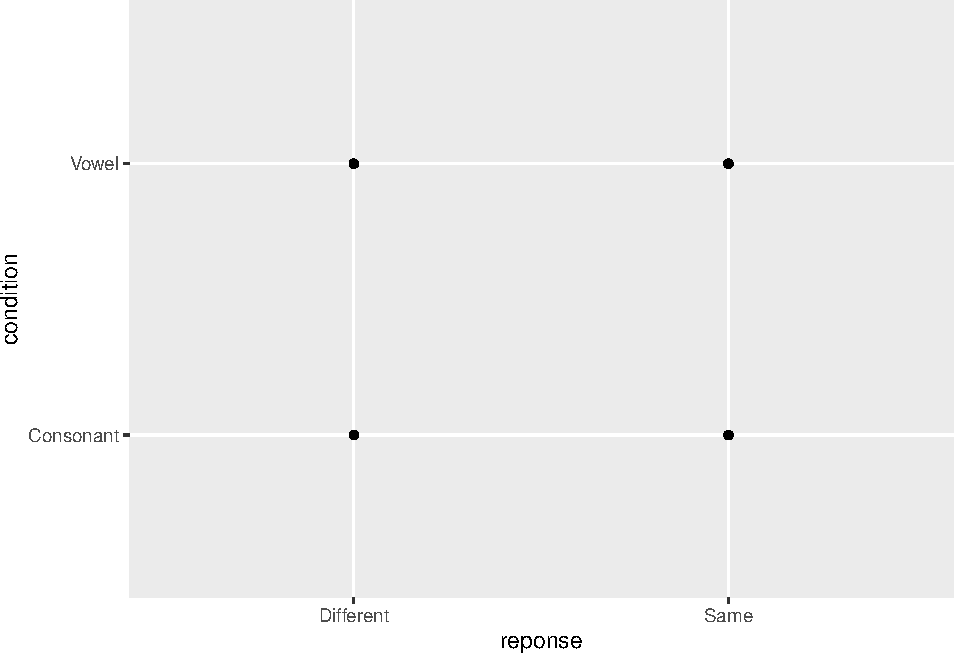
\includegraphics{analysis_files/figure-latex/e2-1-1.pdf}

\hypertarget{exercise-2.2}{%
\subsubsection{Exercise 2.2}\label{exercise-2.2}}

\begin{Shaded}
\begin{Highlighting}[]
\NormalTok{data\_e2\_2 }\OtherTok{\textless{}{-}} \FunctionTok{read\_csv}\NormalTok{(}\StringTok{"data/data\_e2\_2.csv"}\NormalTok{)}
\end{Highlighting}
\end{Shaded}

\begin{verbatim}
## Rows: 1035 Columns: 2
## -- Column specification --------------------------------------------------------
## Delimiter: ","
## chr (1): voicing
## dbl (1): vot
## 
## i Use `spec()` to retrieve the full column specification for this data.
## i Specify the column types or set `show_col_types = FALSE` to quiet this message.
\end{verbatim}

\begin{Shaded}
\begin{Highlighting}[]
\NormalTok{data\_e2\_2 }\SpecialCharTok{\%\textgreater{}\%}
  \FunctionTok{ggplot}\NormalTok{(}\FunctionTok{aes}\NormalTok{(vot, }\AttributeTok{fill =}\NormalTok{ voicing)) }\SpecialCharTok{+}
  \FunctionTok{geom\_bar}\NormalTok{()}
\end{Highlighting}
\end{Shaded}

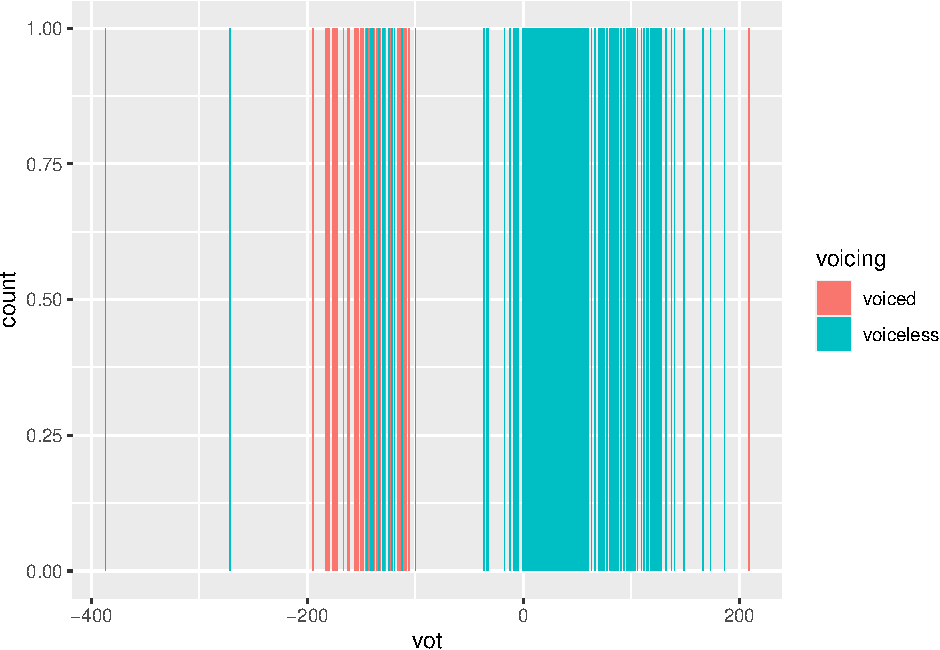
\includegraphics{analysis_files/figure-latex/e2-2-1.pdf}

\hypertarget{exercise-3}{%
\subsection{Exercise 3}\label{exercise-3}}

\begin{itemize}
\tightlist
\item
  Read the \texttt{data\_ex\_3.csv} file in R and obtain summary
  measures (central tendency: mean, median, or mode; and dispersion:
  standard deviation or range) for each variable in the data.
\item
  Make sure to pick the correct measure depending on the variable type.
\item
  For each variable, state the type of variable and the chosen measures
  and report the value of the measures.
\item
  Feel free to add more code chunks as needed.
\end{itemize}

\hypertarget{exercise-4}{%
\subsection{Exercise 4}\label{exercise-4}}

\begin{itemize}
\tightlist
\item
  For each of the variables in the table, specify in the
  \texttt{Probability\ distribution} column whether it's (in principle)
  distributed according to a Gaussian, log-normal, Bernoulli, Poisson
  distribution or to a different distribution (put ``other'' in this
  case).
\item
  If you have doubts about any of the variables, write about it in your
  words below.
\end{itemize}

\begin{longtable}[]{@{}lll@{}}
\toprule\noalign{}
& Variable & Probability distribution \\
\midrule\noalign{}
\endhead
\bottomrule\noalign{}
\endlastfoot
1 & Vowel duration (ms) & \\
2 & Formant values (hz) & \\
3 & Accuracy (binary) & \\
4 & Readability (0-100) & \\
5 & Reaction times (ms) & \\
6 & Number of relative clauses & \\
7 & Scots vs English & \\
8 & Counts of infant gestures & \\
9 & Logged reaction times & \\
10 & Ratio of 1st vs non-1st pronouns & \\
\end{longtable}

\hypertarget{exercise-5}{%
\subsection{Exercise 5}\label{exercise-5}}

\begin{itemize}
\tightlist
\item
  Look at the following table that represents the coding of a
  categorical predictor \texttt{background}.
\item
  Assume treatment coding has been used and that the default
  alphabetical order was intended for the order of the levels.
\item
  Explain what is wrong with the table and write a new table with your
  solution (you can use
  \url{https://tablesgenerator.com/markdown_tables\#} to format the
  markdown table).
\end{itemize}

\begin{longtable}[]{@{}llll@{}}
\toprule\noalign{}
& Bangladeshi & Mandarin & English \\
\midrule\noalign{}
\endhead
\bottomrule\noalign{}
\endlastfoot
Bangladeshi & 1 & 0 & 0 \\
Mandarin & 0 & 2 & 0 \\
English & 0 & 0 & 3 \\
\end{longtable}

\hypertarget{exercise-6}{%
\subsection{Exercise 6}\label{exercise-6}}

Imagine you run the following study:

Participants are asked to listen to nonce words and choose whether they
think the word refers to a small or a big object. Half of the words are
of the \texttt{kiki} type (back consonants and high front vowels), while
half are of the \texttt{baba} type (front consonant and low vowels). The
expectation is that \texttt{kiki} words should elicit more
\texttt{small} responses and \texttt{baba} words more \texttt{big}
responses. We also recorder reaction time and we expect shorter reaction
times to correlate with a greater effect of hearing a \texttt{kiki} word
vs a \texttt{baba} word.

Read the \texttt{data\_e7.csv} file. It contains the following columns:

\begin{itemize}
\tightlist
\item
  \texttt{subject}: the subject's ID.
\item
  \texttt{response}: whether the subject has chosen \texttt{small} or
  \texttt{big}.
\item
  \texttt{condition}: \texttt{kiki} vs \texttt{baba} word.
\item
  \texttt{RT}: reaction time in ms.
\end{itemize}

Make sure to change columns to factors if needed and to specify the
order of levels.

Run a linear model that helps you answer the following questions:

\begin{enumerate}
\def\labelenumi{\arabic{enumi}.}
\tightlist
\item
  Do \texttt{baba} words elicit more \texttt{big} responses than
  \texttt{kiki} words?
\item
  Is the effect of \texttt{baba} words on response greater with shorter
  reaction times?
\end{enumerate}

Report the model specification and the results. Also include a plot of
the model results.

\hypertarget{exercise-7}{%
\subsection{Exercise 7}\label{exercise-7}}

Imagine you are asked to review a paper. Below you can find the
description of a mock study, including the details of the linear model
the researchers have run. The results are not included.

\begin{quote}
We recorded 50 subjects while they read 100 sentences on a screen. For
each subject, half of the sentences were presented together with
pictures of natural landscapes. The other half was presented together
with pictures of urban landscapes. Background sounds were delivered via
headphones to the subject in each trial of the natural and urban setting
condition. For each setting (natural vs urban), half of the trials had
natural sounds (birds, waterfalls, wind, waves, thunders) and half had
urban sounds (traffic noise, sirens, people walking).
\end{quote}

\begin{quote}
For each trial we measured speech rate as number of syllables per second
(syl/s). The hypothesis is that speech rate will be faster in the urban
setting trials relative to the natural setting trials. Moreover, the
effect of background noise (natural vs urban sounds) will decrease
speech rate in the natural setting but not in the urban setting. In
other words, we expect the visual setting (natural vs urban) to prime
speakers to slow down their speech rate, but we expect the auditory
setting (natural vs urban) to make a difference only in the visual
natural setting.
\end{quote}

\begin{quote}
To assess these expectations, we ran a linear model using a Gaussian
distribution with visual setting (natural vs urban) as the outcome
variable. We included the following predictors: speech rate (centred)
and auditory setting (natural vs urban). In R syntax:
\texttt{lm(visual\ \textasciitilde{}\ speech\_rate\_c\ +\ auditory)}.
\end{quote}

Now criticise the analysis (i.e.~explain what is wrong with it) and run
a more appropriate linear model to assess the research hypotheses of the
study based on the provided data (\texttt{data\_e8.csv}). Report the
model specification and results of your linear model.

\hypertarget{exercise-8}{%
\subsection{Exercise 8}\label{exercise-8}}

\begin{itemize}
\tightlist
\item
  Read the 15 statements below.
\item
  For each, indicate whether the statement is true or false by adding an
  ``x'' in the relevant column of the table below.
\end{itemize}

\textbf{Statements}

\begin{enumerate}
\def\labelenumi{\arabic{enumi}.}
\tightlist
\item
  Frequentist CIs and Bayesian CrIs have the same interpretation.
\item
  The types of predictor variables in a linear model decide which
  distribution family to use in the model.
\item
  Strip charts are among the plots that can be used to visualise the
  individual observations of a continuous variable.
\item
  A study result is \emph{robust} when a very similar result is obtained
  with the same data but a different analysis.
\item
  The population-level effects returned by a model summary are
  conditional posterior probabilities.
\item
  Sum-coding a predictor sets the model intercept to the grand mean
  across the levels of that predictor.
\item
  95\% CrIs are more important than 60\% CrIs.
\item
  Quantitative methods are an objective enterprise.
\item
  The most appropriate distribution family for a binary variable is the
  Bernoulli family.
\item
  About 68\% of the data in a Gaussian distribution is contained within
  the range marked by ``mean - 1 SD'' and ``mean + 1 SD''.
\item
  \texttt{plogis(0.3\ +\ 0.2)} is equivalent to
  \texttt{plogis(0.3)\ +\ plogis(0.2)}.
\item
  The goal of statistics is to test for statistical significance.
\item
  When creating a density plot, the \emph{y}-axis can be interpreted as
  the absolute probability of obtaining a specific value.
\item
  Reproducibility and replicability are the same thing.
\item
  The number of parameters to estimate in a model is equivalent to the
  number of predictors in the model.
\end{enumerate}

\textbf{TRUE or FALSE}

\begin{longtable}[]{@{}lll@{}}
\toprule\noalign{}
& True & False \\
\midrule\noalign{}
\endhead
\bottomrule\noalign{}
\endlastfoot
1 & & \\
2 & & \\
3 & & \\
4 & & \\
5 & & \\
6 & & \\
7 & & \\
8 & & \\
9 & & \\
10 & & \\
11 & & \\
12 & & \\
13 & & \\
14 & & \\
15 & & \\
\end{longtable}

\hypertarget{exercise-9}{%
\subsection{Exercise 9}\label{exercise-9}}

\begin{itemize}
\tightlist
\item
  Explain why it is important to include interactions between predictors
  when including multiple predictors in a model.
\end{itemize}

\end{document}
